\documentclass[fleqn]{article}
\usepackage[utf8]{inputenc}
\usepackage{graphicx}
\usepackage{geometry}
\usepackage{svg}
\usepackage[fleqn]{amsmath}
\usepackage{tikz}
\usepackage{grffile}
\usepackage{hyperref}
\usepackage{epstopdf}
\usepackage{longtable}
\graphicspath{{/media/arul/envision/jan-may-2016/kernelmethods/Assignment-1/report/pics}}
\newgeometry{left=3cm, top=2cm, bottom=2cm}
\newcommand{\noimage}{%
  \setlength{\fboxsep}{-\fboxrule}%
  \fbox{\phantom{\rule{150pt}{100pt}}}% Framed box
}
\newcommand{\myparagraph}[1]{\paragraph{#1}\mbox{}\\}
\pagenumbering{gobble}

\title{CS6011 Kernel Methods for Pattern Analysis\\ Assignment-2 \\C-SVM, $\nu$-SVM, Convolutional Neural Network, RBM}
\author{Arulkumar S (CS15S023), Divya Saglani (CS15M041), Nitish (CS15S028)}

\date{3rd March 2016}

\begin{document}
\setcounter{secnumdepth}{5}
\tracingall
\maketitle

\section{Introduction}
\section{Analysis of SVM with 2D data}
\section{PCA, Auto-encoder, Stacked Auto-encoder}

\newpage
\section{Deep convolutional neural network (DCNN)}

\subsection{Model}
The model skeleton is shown below.\\\\
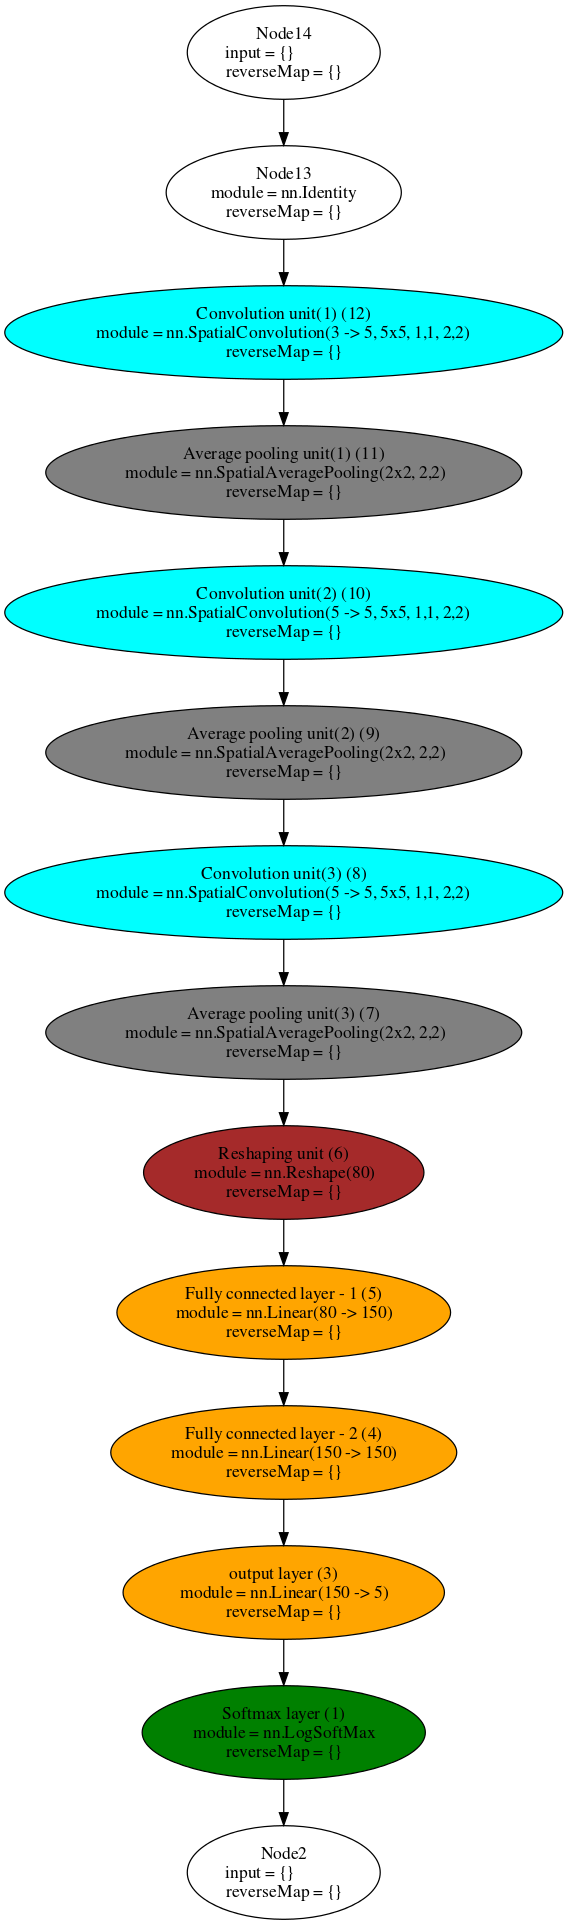
\includegraphics[scale=0.3]{./pics/filt=5-hidden1=5-hidden2=5-hidden3=5-fc1=150-fc2=150}
\newpage
The model consists of three sets of ``convolution + average pooling'' layers followed by two Fully connected layers and output layer.
The output layer gives Softmax output (5 nodes) for each class.\\\\

The model is trained using Stochastic Gradient Descent optimization technique with the following parameters.\\

\begin{itemize}
  \item Learning Rate = 0.02
  \item Batch Size = 128
  \item Weight decay = $5e^{-4}$
  \item Momentum = 0.9
\end{itemize}

\subsection{Data}

The given image data (of size 200 x 200 pixels) are resized into 32 x 32 pixels sized images and splitted into Training (75\%), Validation(12.5\%) and Test(12.5\%) set. \\

Total number of images given are: \\

\begin{itemize}
  \item cow: 302 (train = 226 images, validation = 38 images, test = 38 images)
  \item boat: 500 (train = 375 images, validation = 62 images, test = 63 images)
  \item sheep: 316 (train = 237 images, validation = 39 images, test = 40 images)
  \item bottle: 757 (train = 567 images, validation = 95 images, test = 95 images)
  \item bird: 753 (train = 564 images, validation = 94 images, test = 95 images)
\end{itemize}

\subsection{Model selection}

\begin{itemize}
  \item The model selection is carried out by varying the ``number of output feature maps'' in 3 convolution layers and ``number of nodes'' 2 Fully connected layers.
  \item For convolution layers, the ``number of output feature maps'' applied are 5, 15. \& the filter sizes applied are 3, 5.
  \item For Fully connected layers, the ``number of nodes'' applied are 150, 300.
  \item Totally, 64 CNNs are trained based on the combinations from Convolution layers and Fully connected layers.
  \item The best model is selected based on the validation accuracy of the trained model.
\end{itemize}

According to validation criteria, the best performing models are found to be,\\

\begin{center}
  \begin{longtable}{c | c | c | c | c | c | c | c | c}
    \multicolumn{1}{c}{Model Number} &
  	\multicolumn{1}{c}{conv1} &
	\multicolumn{1}{c}{conv2} & 
	\multicolumn{1}{c}{conv3} & 
	\multicolumn{1}{c}{filter-size } & 
	\multicolumn{1}{c}{FC1} &
	\multicolumn{1}{c}{FC2} & 
	\multicolumn{1}{c}{Training(\%)} &
	\multicolumn{1}{c}{Validation(\%)}\\
	\hline
    1  &  5       &  15    &  15     & 5    &  150    &  150 		& 51.142 & 53.048\\\hline 
    2  &  5      &   15     &  5    &  5    &  300    & 150 		& 50.634 & 53.048\\\hline
	
  \end{longtable}
\end{center}

The above models will be referred as \textbf{model-1} \& \textbf{model-2} respectively in upcoming pages.

\subsection{Confusion matrices}

\subsubsection{Model-1 (after 167 epochs)}
\myparagraph{Training set}
\begin{center}
  \begin{longtable}{ c | c | c | c | c | c | c}
  	\multicolumn{1}{c}{} &
	\multicolumn{1}{c}{cow} & 
	\multicolumn{1}{c}{boat } & 
	\multicolumn{1}{c}{sheep } &
	\multicolumn{1}{c}{bottle } & 
	\multicolumn{1}{c}{bird } &
	\multicolumn{1}{c}{Total correct (\%) }\\
    \hline
    cow       &  70    &  26     & 11    &  52    &  67         & 30.973\\\hline 
    boat      &  5     & 222     &  1    &  46    & 101         & 59.200\\\hline
    sheep     &  33    &  31     & 21    &  55    &  97         & 8.861\\\hline
    bottle    &   8    &  44     &  5    & 399    & 111         & 70.370\\\hline
    bird      &  19    &  83     & 19    & 148    & 295         & 52.305\\\hline
              &      &         &        &        &   Accuracy 	& 51.142\\\hline
  \end{longtable}
\end{center}

\myparagraph{Validation set}

\begin{center}
  \begin{longtable}{ c | c | c | c | c | c | c}
  	\multicolumn{1}{c}{} &
	\multicolumn{1}{c}{cow} & 
	\multicolumn{1}{c}{boat } & 
	\multicolumn{1}{c}{sheep } &
	\multicolumn{1}{c}{bottle } & 
	\multicolumn{1}{c}{bird } &
	\multicolumn{1}{c}{Total correct (\%) }\\
    \hline
    cow       &  9   &    5    &    4   &    9    &     11      &   23.684\\\hline 
    boat      &  3   &   39    &    1   &   12    &      7      &   62.903\\\hline
    sheep     &  2   &    6    &   12   &    9    &     10      &   30.769\\\hline
    bottle    &  1   &   11    &    3   &   64    &     16      &   67.368\\\hline
    bird      &  3   &   11    &    5   &   25    &     50      &   53.191\\\hline
              &      &         &        &         &   Accuracy 	&   53.048\\\hline
  \end{longtable}
\end{center}

\myparagraph{Test set}

\begin{center}
  \begin{longtable}{ c | c | c | c | c | c | c}
  	\multicolumn{1}{c}{} &
	\multicolumn{1}{c}{cow} & 
	\multicolumn{1}{c}{boat } & 
	\multicolumn{1}{c}{sheep } &
	\multicolumn{1}{c}{bottle } & 
	\multicolumn{1}{c}{bird } &
	\multicolumn{1}{c}{Total correct (\%) }\\
    \hline
    cow       &  12    &    5    &    2     &   7    &   12     &   31.579\\\hline 
    boat      &  2     &   29    &    0     &   6    &   26     &   46.032\\\hline
    sheep     &  11    &    6    &    5     &   7    &   11     &   12.500\\\hline
    bottle    &  2     &    9    &    0     &   71   &   13     &   74.737\\\hline
    bird      &  4     &    12   &    2     &   30   &   47     &  49.474\\\hline
              &        &         &          &        & Accuracy & 49.546\\\hline
  \end{longtable}
\end{center}

\newpage
\subsubsection{Model-2 (after 183 epochs)}
\myparagraph{Training set}
\begin{center}
  \begin{longtable}{ c | c | c | c | c | c | c}
  	\multicolumn{1}{c}{} &
	\multicolumn{1}{c}{cow} & 
	\multicolumn{1}{c}{boat } & 
	\multicolumn{1}{c}{sheep } &
	\multicolumn{1}{c}{bottle } & 
	\multicolumn{1}{c}{bird } &
	\multicolumn{1}{c}{Total correct (\%) }\\
    \hline
    cow       &  68    &  30     & 17    &  55    &  56 		& 30.088\\\hline 
    boat      &  9     &  213    &  3    &  41    & 109 		& 56.800\\\hline
    sheep     &  31    &  27     & 34    &  62    &  83 		& 14.346\\\hline
    bottle    &   8    &  46     &  9    & 397    & 107 		& 70.018\\\hline
    bird      &  20    &  82     & 25    & 152    & 285 		& 50.532\\\hline
              &      &         &        &        &   Accuracy 	& 50.634\\\hline
  \end{longtable}
\end{center}

\myparagraph{Validation set}

\begin{center}
  \begin{longtable}{ c | c | c | c | c | c | c}
  	\multicolumn{1}{c}{} &
	\multicolumn{1}{c}{cow} & 
	\multicolumn{1}{c}{boat } & 
	\multicolumn{1}{c}{sheep } &
	\multicolumn{1}{c}{bottle } & 
	\multicolumn{1}{c}{bird } &
	\multicolumn{1}{c}{Total correct (\%) }\\
    \hline
    cow       &  10  &    3    &    4   &    10   &   	11 		& 26.316\\\hline 
    boat      &  3   &   32    &    2   &    15   &   	10 		& 51.613\\\hline
    sheep     &  2   &    6    &   11   &    8    &   	12 		& 28.205\\\hline
    bottle    &  1   &    8    &    2   &    66   &   	18 		& 69.474\\\hline
    bird      &  2   &   10    &    3   &    24   &   	55 		& 58.511\\\hline
              &      &         &        &         &   Accuracy 	& 53.048\\\hline
  \end{longtable}
\end{center}
 
\myparagraph{Test set}

\begin{center}
  \begin{longtable}{ c | c | c | c | c | c | c}
  	\multicolumn{1}{c}{} &
	\multicolumn{1}{c}{cow} & 
	\multicolumn{1}{c}{boat } & 
	\multicolumn{1}{c}{sheep } &
	\multicolumn{1}{c}{bottle } & 
	\multicolumn{1}{c}{bird } &
	\multicolumn{1}{c}{Total correct (\%) }\\
    \hline
    cow       &  11     &  2     &  3   &    7   &   15     & 28.947\\\hline 
    boat      &  2      & 29     &  0   &    6   &   26     & 46.032\\\hline
    sheep     &  8      &  4     & 10   &    6   &   12     & 25.000\\\hline
    bottle    &  3      &  6     &  0   &   71   &   15     & 74.737\\\hline
    bird      &  3      & 12     &  3   &   29   &   48     & 50.526\\\hline
              &         &        &      &        & Accuracy & 51.057\\\hline
  \end{longtable}
\end{center}

\subsection{Training and validation accuracy}
During training phase, after each epoch of training, the accuracy of validation set is being noted down to detect overfitting on the training data.
As shown in the picture, the model starts to overfit on the training data after certain epoch (~180 epochs). 
So, it is important to keep track of validation accuracy and select the appropriate model for testing.\\  
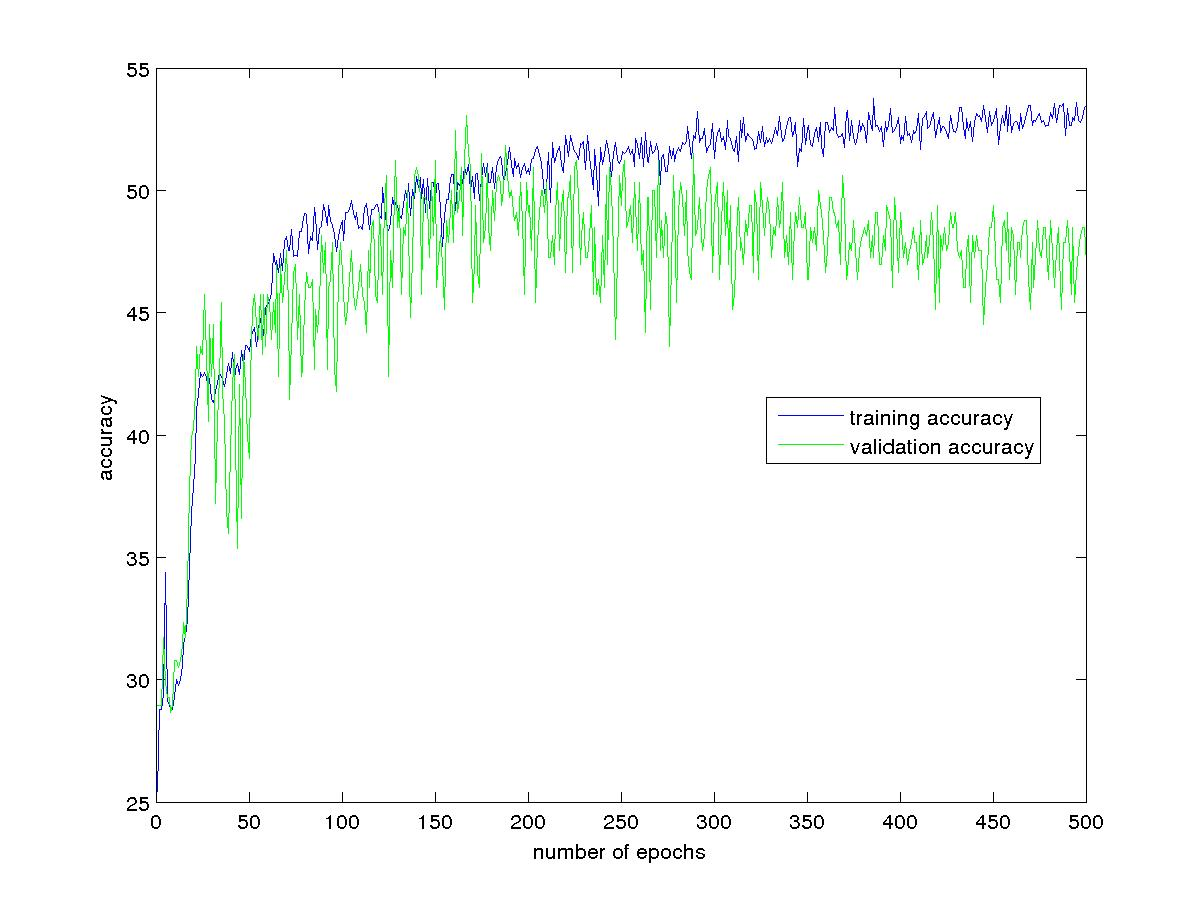
\includegraphics[scale=0.4]{../src/imageclassification/bestmodels/filt=5-hidden1=5-hidden2=15-hidden3=5-fc1=300-fc2=150/accuracy_trend.jpg}\\

\subsubsection{Observations}

\begin{itemize}
  \item During initial epochs of training, the model is biased with the classes having more data (bottle, bird) and predicts only those classes (bottle, bird) for all the data.
Once, the gradient is backpropagated for multiple epochs (~20 epochs), the model starts to learn all other classes.
 \item Due to the imbalance in the data, the classes which has more data (bottle, bird) are learned effectively than the classes having less data.
  \item For 3 convolution layers, the model is overfitting after \textasciitilde180 epochs. It can be accounted to the fact that only less amount of data is available for training.
\end{itemize}

\subsection{Convolution layer-1 filters (Model-1)}
The visualization of convolution layer-1 filters is shown below.
From the filters, it can be inferred that the first convolution layer filters learn the color information (mainly, green, reddish, blue colors) in the training images.\\
\includegraphics[scale=0.6]{./pics/conv1_filters.png}\\

\subsection{Hidden layer output visualization}
The output of convolution layers for each class image(s) is shown below.
As we can see in the layer outputs, the initial convolution nodes are able to learn low level features such as Edges, 
the second convolution layer is able to give high activation value when a particular object is found.
The linear fully connected layers are acting as classifiers for the classes based on the learned features from convolution layers.

\subsubsection{Model-1}
\myparagraph{class 'cow'}
\includegraphics[scale=0.6]{./pics/model1_cow_hidden_layers.png}\\
\myparagraph{class 'boat'}
\includegraphics[scale=0.6]{./pics/model1_boat_hidden_layers.png}\\
\myparagraph{class 'sheep'}
\includegraphics[scale=0.6]{./pics/model1_sheep_hidden_layers.png}\\
\myparagraph{class 'bottle'}
\includegraphics[scale=0.6]{./pics/model1_bottle_hidden_layers.png}\\
\myparagraph{class 'bird'}
\includegraphics[scale=0.6]{./pics/model1_bird_hidden_layers.png}

\subsubsection{Model-2}
\myparagraph{class 'cow'}
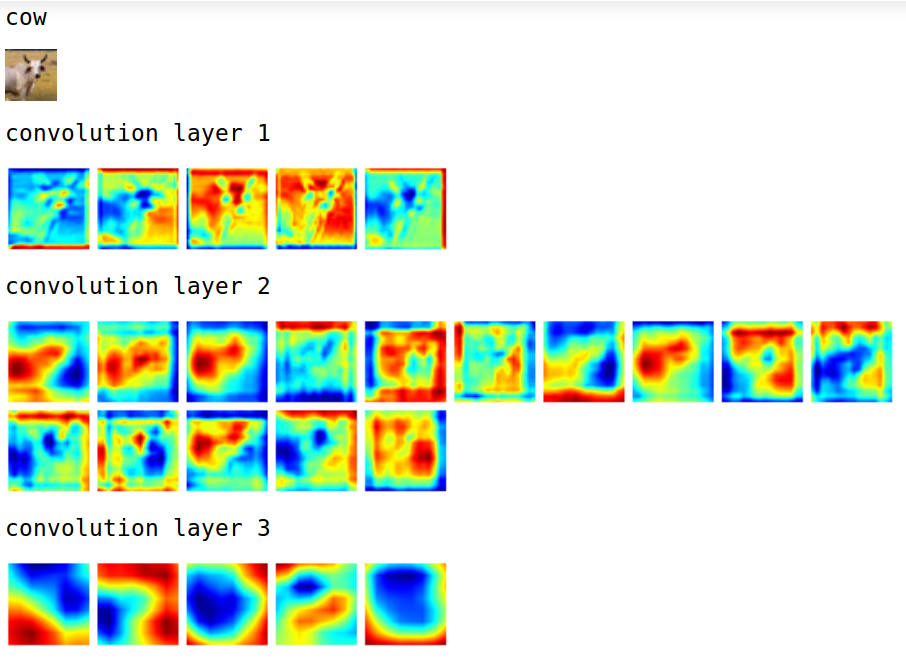
\includegraphics[scale=0.4]{./pics/cow_hidden_layers.png}\\
\myparagraph{class 'boat'}
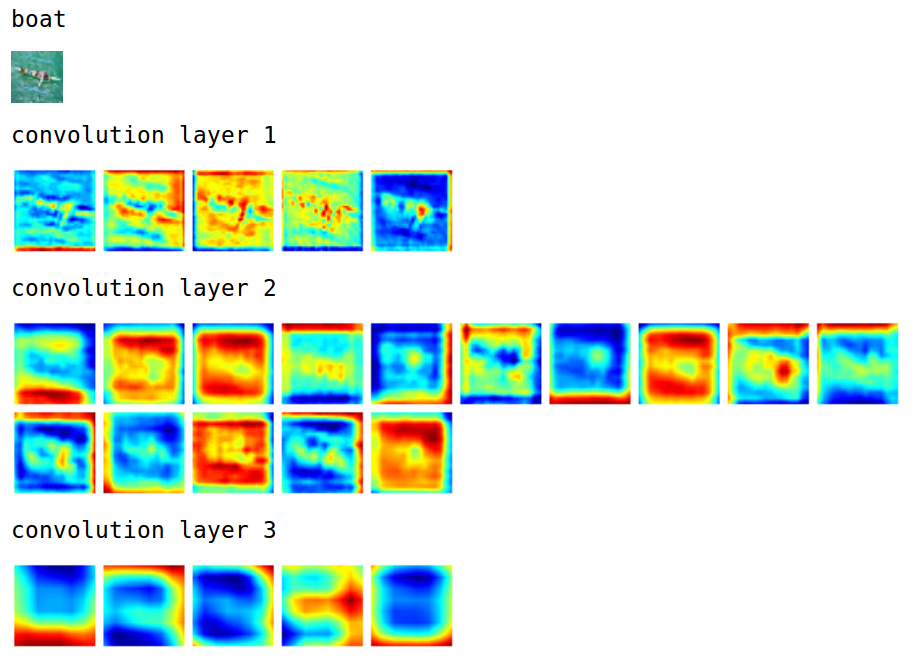
\includegraphics[scale=0.4]{./pics/boat_hidden_layers.png}\\
\myparagraph{class 'sheep'}
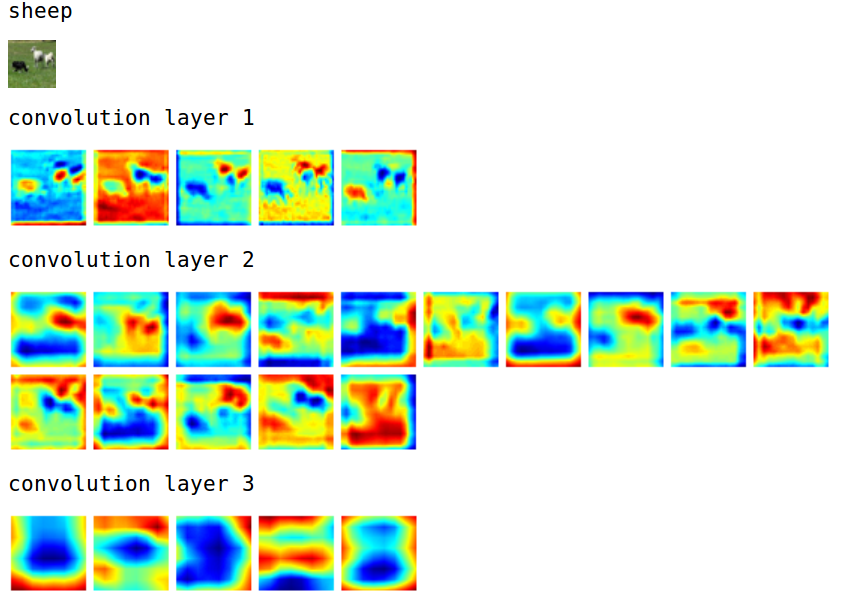
\includegraphics[scale=0.4]{./pics/sheep_hidden_layers.png}\\
\myparagraph{class 'bottle'}
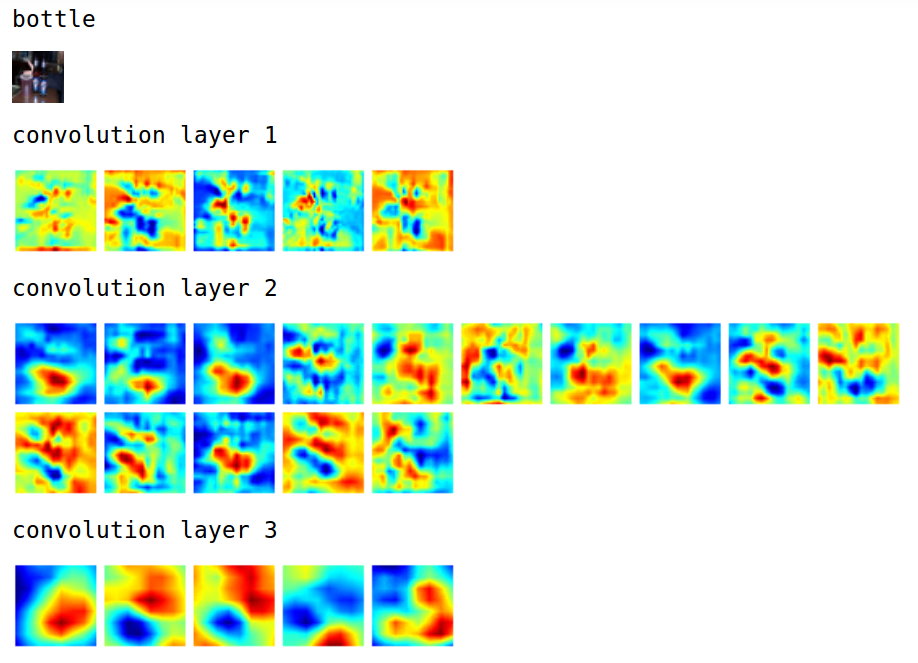
\includegraphics[scale=0.4]{./pics/bottle_hidden_layers.png}\\
\myparagraph{class 'bird'}
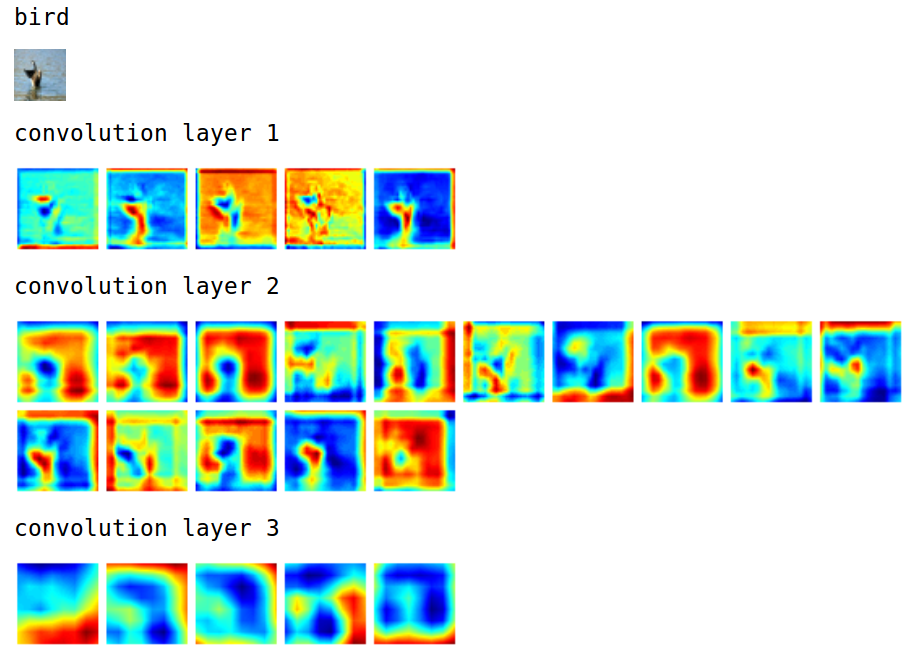
\includegraphics[scale=0.4]{./pics/bird_hidden_layers.png}

It can be clearly noticed from the convolution layer outputs (especially from conv2), the model is able to locate the object and provide higher activation value on object's location.\\

\subsection{A closer look at misclassified images}

\subsubsection{actual: 'cow' \& predicted : 'boat'}

\includegraphics[scale=1.5]{./pics/miscallssify_cow_to_boat.png}\\

\subsubsection{actual: 'boat' \& predicted : 'cow'}

\includegraphics[scale=1.5]{./pics/miscallssify_boat_to_cow.png}\\

\subsubsection{actual: 'cow' \& predicted : 'bird'}
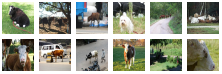
\includegraphics[scale=1.5]{./pics/miscallssify_cow_to_bird.png}\\

\subsubsection{actual: 'bird' \& predicted: 'cow'}
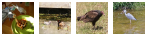
\includegraphics[scale=1.5]{./pics/miscallssify_bird_to_cow.png}\\

\subsubsection{actual: 'bird' \& predicted : 'boat'}
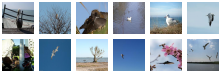
\includegraphics[scale=1.5]{./pics/miscallssify_bird_to_boat.png}\\

\subsubsection{actual: 'boat' \& predicted : 'bird'}
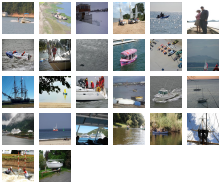
\includegraphics[scale=1.5]{./pics/miscallssify_boat_to_bird.png}

It can be inferred from the images that the 'boat' and 'bird' classes contain 'blue' color in most of their pictures which makes the model to misclassify these images.\\

\subsubsection{actual: 'cow' \& predicted : 'sheep'}
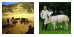
\includegraphics[scale=1.5]{./pics/miscallssify_cow_to_sheep.png}\\

\subsubsection{actual: 'sheep' \& predicted : 'cow'}
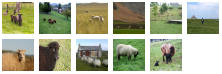
\includegraphics[scale=1.5]{./pics/miscallssify_sheep_to_cow.png}\\

\subsubsection{actual: 'bird' \& predicted : 'sheep'}
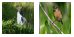
\includegraphics[scale=1.5]{./pics/miscallssify_bird_to_sheep.png}\\

\subsubsection{actual: 'sheep' \& predicted : 'bird'}
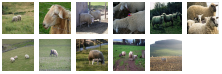
\includegraphics[scale=1.5]{./pics/miscallssify_sheep_to_bird.png}\\

\subsubsection{actual: 'bottle' \& predicted : 'cow'}

\includegraphics[scale=1.5]{./pics/miscallssify_bottle_to_cow.png}\\

\subsubsection{actual: 'cow' \& predicted : 'bottle'}
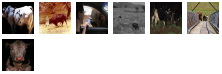
\includegraphics[scale=1.5]{./pics/miscallssify_cow_to_bottle.png}\\

\subsubsection{actual: 'bird' \& predicted : 'bottle'}
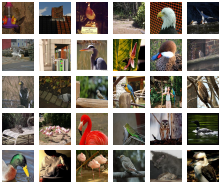
\includegraphics[scale=1.5]{./pics/miscallssify_bird_to_bottle.png}\\

\subsubsection{actual: 'bottle' \& predicted : 'bird'}
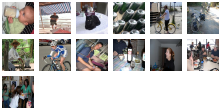
\includegraphics[scale=1.5]{./pics/miscallssify_bottle_to_bird.png}\\

\subsubsection{actual: 'boat' \& predicted : 'bottle'}

\includegraphics[scale=1.5]{./pics/miscallssify_boat_to_bottle.png}\\

\subsubsection{actual: 'bottle' \& predicted : 'boat'}
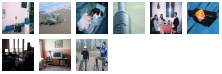
\includegraphics[scale=1.5]{./pics/miscallssify_bottle_to_boat.png}\\

\subsubsection{actual: 'sheep' \& predicted : 'bottle'}
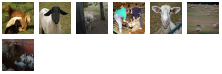
\includegraphics[scale=1.5]{./pics/miscallssify_sheep_to_bottle.png}\\

\subsubsection{actual: 'sheep' \& predicted : 'boat'}
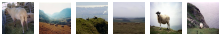
\includegraphics[scale=1.5]{./pics/miscallssify_sheep_to_boat.png}\\

\subsection{Effect of Data augmentation strategies}

\begin{itemize}
  \item Since the data set is imbalanced (i.e., class 'bird' has double the data of class 'cow'), we tried to balance it by using Label preserving transformations.
 During data augmentation, the original images are translated randomly by [-0.1H to +0.1H] (i.e., 3 pixels) and each image is also horizontally flipped.
 \item After the data augmentation, the number of images is increased to \textasciitilde20000 with \textasciitilde3000 images per class.
 the model (conv1=5, conv2=15, conv3=15, FC1=150, FC2=150) is trained using the augmented dataset and the validation performance is measured.
 Eventhough, we increase the data by augmenting, the training accuracy (48\%) and validation accuracy (46\%) are not increased.
\end{itemize}

\newpage
\section{$\nu$-SVM classification using DCNN features}
The DCNN features output from Fully connected layer-2 (150 dimensional data) of Model-1 is considered for classification using $\nu$-SVM.\\\\
$\nu-SVM$ from the package ``LibSVM'' is used to classify the features obtained from DCNN.

\subsection{Accuracy: $\nu$ vs RBF scale factor(gamma)}
\subsubsection{Training accuracy}
\includegraphics[scale=0.3]{./pics/imagesvc/nu-SVM Classification using DCNN featurestrain_accuracy.jpg}\\
\subsubsection{Validation accuracy}
\includegraphics[scale=0.3]{./pics/imagesvc/nu-SVM Classification using DCNN featuresvalidation_accuracy.jpg}\\

\subsection{Parameter selection}
From the training accuracy, validation accuracy images, we can notice that

\begin{itemize}
  \item when the $\nu$ parameter is increased (to \textasciitilde0.5), we are allowing more outliers, inturn the number of support vectors is increased.
  \item We need to find the balance between the number of support vectors and the accuracy. 
  usually, $\nu = 0.05$ to $0.3$ is preferred. So we shall choose a model which gives greater performance on validation set with $0.05 <= \nu <= 0.3$ 
  \item From the images, it can be seen that when $\nu$ is very small (\textasciitilde0.06) \& gamma is high, the model tries to fit training data perfectly (i.e., overfit).
  It is confirmed by looking at validation accuracy. Eventhough, training accuracy is >95\%, validation accuracy is not increased. 
\end{itemize}

The below parameters are choosen based on validation set performance of various models.

\begin{itemize}
  \item $\nu$ = 0.26
  \item RBF kernel scale factor (gamma) = 0.02
\end{itemize}

\subsection{Confusion matrices}
\myparagraph{Training set}
\begin{center}
  \begin{longtable}{ c | c | c | c | c | c }
  	\multicolumn{1}{c}{} &
	\multicolumn{1}{c}{cow} & 
	\multicolumn{1}{c}{boat } & 
	\multicolumn{1}{c}{sheep } &
	\multicolumn{1}{c}{bottle } & 
	\multicolumn{1}{c}{bird } \\
    \hline
    cow       &  	171  &  9 	&  	1  	& 24 	& 21		\\\hline 
    boat      & 	6 	 & 	313 & 	4 	& 21 	& 31		\\\hline
    sheep     &  	0  	& 	17  & 	174 & 21 	& 25\\\hline
    bottle    &  	1 	& 	14 	& 	4 	& 519 	& 29\\\hline
    bird      & 	4 	& 	15	&   6 	& 16	& 523\\\hline
              &        &      &        &   Accuracy 	& 86.33\\\hline
  \end{longtable}
\end{center}

\myparagraph{Validation set}

\begin{center}
  \begin{longtable}{ c | c | c | c | c | c }
  	\multicolumn{1}{c}{} &
	\multicolumn{1}{c}{cow} & 
	\multicolumn{1}{c}{boat } & 
	\multicolumn{1}{c}{sheep } &
	\multicolumn{1}{c}{bottle } & 
	\multicolumn{1}{c}{bird } \\
    \hline
    cow       &  	11  &   4 	&  	5  	& 6 	& 12		\\\hline 
    boat      & 	7 	 & 	29 & 	2 	& 12 	& 12		\\\hline
    sheep     &  	5  	& 	6  & 	13 & 5 	& 10\\\hline
    bottle    &  	6 	& 	15 	& 	6 	& 47 	& 21\\\hline
    bird      & 	11 	& 	17	&   2 	& 22	& 42\\\hline
              &        &      &        &   Accuracy 	& 43.297\\\hline
  \end{longtable}
\end{center}
 
\myparagraph{Test set}

\begin{center}
  \begin{longtable}{ c | c | c | c | c | c }
  	\multicolumn{1}{c}{} &
	\multicolumn{1}{c}{cow} & 
	\multicolumn{1}{c}{boat } & 
	\multicolumn{1}{c}{sheep } &
	\multicolumn{1}{c}{bottle } & 
	\multicolumn{1}{c}{bird } \\
    \hline
    cow       &  	10  &   5 	&  	7  	& 12 	& 4		\\\hline 
    boat      & 	3 	 & 	35 & 	3	& 5 	& 17		\\\hline
    sheep     &  	7  	& 	8  & 	9   & 3 	& 13\\\hline
    bottle    &  	6	& 	12 	& 	5	& 61 	& 11\\\hline
    bird      & 	6 	& 	13	&   7 	& 21	& 48\\\hline
              &        &      &        &   Accuracy 	& 49.245\\\hline
  \end{longtable}
\end{center}

\subsection{Observations}

\begin{itemize}
  \item when $\nu$ is very less (\textasciitilde0.05), the model tends to overfit on training data.
  \item When $\nu$ is increased, the number of support vectors, as well as the accuracy on validation data increases, due to the fact that we are allowing more outliers. 
\end{itemize}

\end{document}